\documentclass[11pt, a4paper]{article}

% Fonts and Encoding
\usepackage[utf8]{inputenc}
\usepackage[T1]{fontenc}

% Math and Symbols
\usepackage{amsmath, amssymb, amsthm, amsfonts, mathrsfs, mathtools}

% Layout and Geometry
\usepackage{geometry}
\geometry{a4paper, margin=1in}

% Formatting and Graphics
\usepackage{graphicx, xcolor, enumitem, booktabs, array, tabularx}

% TikZ for Illustrations
\usepackage{tikz}
\usetikzlibrary{arrows.meta, positioning, shapes.geometric, calc, backgrounds, matrix}

% Clickable Links and TOC
\usepackage{hyperref}
\hypersetup{
    colorlinks=true,
    linkcolor=blue,
    filecolor=magenta,      
    urlcolor=cyan,
    pdftitle={Advanced Mathematics Topic},
}

% Theorem Environments
\newtheorem{theorem}{Theorem}[section]
\newtheorem{lemma}[theorem]{Lemma}
\newtheorem{proposition}[theorem]{Proposition}
\newtheorem{corollary}[theorem]{Corollary}
\theoremstyle{definition}
\newtheorem{definition}{Definition}[section]
\newtheorem{axiom}{Axiom}[section]
\newtheorem{example}{Example}[section]
\theoremstyle{remark}
\newtheorem{remark}{Remark}[section]

% Custom Commands (Enforced standard notation)
\newcommand{\R}{\mathbb{R}}
\newcommand{\N}{\mathbb{N}}
\newcommand{\Z}{\mathbb{Z}}
\newcommand{\Q}{\mathbb{Q}}
\newcommand{\E}{\mathbb{E}}
\newcommand{\Prob}{\mathbb{P}}
\newcommand{\F}{\mathcal{F}}

\title{Higher-Order Linear Homogeneous Differential Equations}
\author{Tashfeen Omran}
\date{October 29, 2026}

\begin{document}

\maketitle
\tableofcontents
\newpage

\section{Part 1: Comprehensive Introduction, Context, and Prerequisites}

\subsection{Core Concepts}
The topic at hand is the study of \textbf{Higher-Order Linear Homogeneous Differential Equations with Constant Coefficients}. A linear differential equation of order $n$ with constant coefficients can be written in the standard form:
\[ a_n y^{(n)} + a_{n-1} y^{(n-1)} + \dots + a_1 y' + a_0 y = 0 \]
where $a_n, a_{n-1}, \dots, a_0$ are real constants, $a_n \neq 0$, and $y^{(k)}$ denotes the $k$-th derivative of the unknown function $y(x)$ with respect to the independent variable $x$. The term ``homogeneous'' indicates that the right-hand side of the equation is zero, meaning the system is unforced and its behavior is dictated entirely by its internal properties and initial conditions.

\subsection{Intuition and Derivation}
The fundamental intuition for solving these equations comes from first-order linear equations, where the solution is an exponential function. We hypothesize that the solution to the higher-order equation takes the form $y(x) = e^{rx}$, where $r$ is a constant to be determined. 

Substituting $y(x) = e^{rx}$ and its derivatives $y^{(k)}(x) = r^k e^{rx}$ into the differential equation yields:
\[ a_n r^n e^{rx} + a_{n-1} r^{n-1} e^{rx} + \dots + a_1 r e^{rx} + a_0 e^{rx} = 0 \]
Factoring out the non-zero term $e^{rx}$, we obtain the \textbf{characteristic equation}:
\[ a_n r^n + a_{n-1} r^{n-1} + \dots + a_1 r + a_0 = 0 \]
This transforms the calculus problem of solving a differential equation into an algebraic problem of finding the roots of an $n$-th degree polynomial. The nature of these roots (real and distinct, real and repeated, or complex conjugates) dictates the fundamental set of solutions.

\subsection{Historical Context and Motivation}
The systematic theory of linear differential equations was largely developed in the 18th century by mathematicians such as Leonhard Euler and Jean le Rond d'Alembert. The motivation stemmed from classical mechanics, specifically the study of vibrating strings, pendulums, and spring-mass systems. Euler was the first to introduce the exponential substitution $y = e^{rx}$ in 1743, recognizing that the derivatives of exponential functions are proportional to the functions themselves, making them the perfect mathematical tool to model systems where the rate of change is proportional to the state of the system.

\subsection{Key Formulas}
Depending on the roots of the characteristic equation, the general solution is constructed using the principle of superposition:
\begin{itemize}
    \item \textbf{Distinct Real Roots:} If $r_1, r_2, \dots, r_k$ are distinct real roots, the corresponding part of the solution is:
    \[ y(x) = c_1 e^{r_1 x} + c_2 e^{r_2 x} + \dots + c_k e^{r_k x} \]
    \item \textbf{Repeated Real Roots:} If a real root $r$ has multiplicity $m$, we multiply by powers of $x$ to ensure linear independence:
    \[ y(x) = (c_1 + c_2 x + c_3 x^2 + \dots + c_m x^{m-1}) e^{rx} \]
    \item \textbf{Complex Conjugate Roots:} If roots are $r = \alpha \pm i\beta$ with multiplicity $m$, Euler's formula ($e^{i\theta} = \cos\theta + i\sin\theta$) transforms the complex exponentials into real-valued functions:
    \[ y(x) = e^{\alpha x} \left[ (c_1 + c_2 x + \dots + c_m x^{m-1})\cos(\beta x) + (d_1 + d_2 x + \dots + d_m x^{m-1})\sin(\beta x) \right] \]
\end{itemize}

\subsection{Prerequisites}
To master this topic, one must be proficient in:
\begin{enumerate}
    \item \textbf{Polynomial Algebra:} Factoring high-degree polynomials, using synthetic division, and applying the Rational Root Theorem.
    \item \textbf{Complex Numbers:} Understanding complex conjugates and Euler's formula.
    \item \textbf{Calculus:} Computing higher-order derivatives, especially using the product rule and chain rule for functions like $x^k e^{\alpha x} \cos(\beta x)$.
    \item \textbf{Linear Algebra:} Solving systems of linear equations to find constants $c_k$ for Initial Value Problems (IVPs).
\end{enumerate}

\newpage
\section{Part 2: Detailed Homework Solutions}

\subsection*{Problem 1}
\textbf{Find a general solution for the given differential equation:}
\[ y''' - 5y'' - 36y' = 0 \]

\textbf{Solution:}
First, we write the characteristic equation:
\[ r^3 - 5r^2 - 36r = 0 \]
Factor out the common term $r$:
\[ r(r^2 - 5r - 36) = 0 \]
Factor the quadratic polynomial. We need two numbers that multiply to $-36$ and add to $-5$. These are $-9$ and $4$:
\[ r(r - 9)(r + 4) = 0 \]
The roots are $r_1 = 0$, $r_2 = 9$, and $r_3 = -4$. Since these are distinct real roots, the general solution is:
\[ y(x) = c_1 e^{0x} + c_2 e^{9x} + c_3 e^{-4x} \]
Simplifying $e^{0x} = 1$, we get the final answer:
\[ y(x) = c_1 + c_2 e^{9x} + c_3 e^{-4x} \]

\subsection*{Problem 2}
\textbf{Find a general solution for the given differential equation:}
\[ y''' - 2y'' - 31y' - 28y = 0 \]

\textbf{Solution:}
The characteristic equation is:
\[ r^3 - 2r^2 - 31r - 28 = 0 \]
We use the Rational Root Theorem to test potential roots (factors of $-28$). Let's test $r = -1$:
\[ (-1)^3 - 2(-1)^2 - 31(-1) - 28 = -1 - 2 + 31 - 28 = 0 \]
Since $r = -1$ is a root, $(r + 1)$ is a factor. We perform polynomial division of $(r^3 - 2r^2 - 31r - 28)$ by $(r + 1)$:
\[ r^3 - 2r^2 - 31r - 28 = (r + 1)(r^2 - 3r - 28) \]
Now, factor the quadratic $r^2 - 3r - 28$. We need numbers that multiply to $-28$ and add to $-3$. These are $-7$ and $4$:
\[ (r + 1)(r - 7)(r + 4) = 0 \]
The roots are $r_1 = -1$, $r_2 = 7$, and $r_3 = -4$. The general solution is:
\[ y(x) = c_1 e^{-x} + c_2 e^{7x} + c_3 e^{-4x} \]

\subsection*{Problem 3}
\textbf{Find a general solution for the given differential equation:}
\[ y''' + y'' - 16y' + 20y = 0 \]

\textbf{Solution:}
The characteristic equation is:
\[ r^3 + r^2 - 16r + 20 = 0 \]
Testing factors of $20$, let's try $r = 2$:
\[ (2)^3 + (2)^2 - 16(2) + 20 = 8 + 4 - 32 + 20 = 0 \]
Thus, $(r - 2)$ is a factor. Dividing the polynomial by $(r - 2)$:
\[ r^3 + r^2 - 16r + 20 = (r - 2)(r^2 + 3r - 10) \]
Factoring the quadratic $r^2 + 3r - 10$ yields $(r - 2)(r + 5)$. The fully factored equation is:
\[ (r - 2)^2 (r + 5) = 0 \]
The roots are $r = 2$ (multiplicity 2) and $r = -5$ (multiplicity 1). Because $r=2$ is repeated, we must multiply the second term by $x$:
\[ y(x) = c_1 e^{2x} + c_2 x e^{2x} + c_3 e^{-5x} \]

\subsection*{Problem 4}
\textbf{Find a general solution for the given differential equation:}
\[ y^{(4)} + 6y'' + 9y = 0 \]

\textbf{Solution:}
The characteristic equation is:
\[ r^4 + 6r^2 + 9 = 0 \]
This is a quadratic in form. Let $u = r^2$. Then $u^2 + 6u + 9 = 0$, which factors as $(u + 3)^2 = 0$. Substituting back $r^2$:
\[ (r^2 + 3)^2 = 0 \]
The roots of $r^2 + 3 = 0$ are $r = \pm i\sqrt{3}$. Because of the square, these complex roots have a multiplicity of 2. 
For $r = 0 \pm i\sqrt{3}$, $\alpha = 0$ and $\beta = \sqrt{3}$. The repeated complex roots require multiplying by $x$:
\[ y(x) = c_1 \cos(\sqrt{3}x) + c_2 \sin(\sqrt{3}x) + c_3 x \cos(\sqrt{3}x) + c_4 x \sin(\sqrt{3}x) \]

\subsection*{Problem 5}
\textbf{Find a general solution for the given differential equation. [Hint: $y(x) = \sin(4x)$ is a solution.]}
\[ y^{(4)} - 2y''' + 17y'' - 32y' + 16y = 0 \]

\textbf{Solution:}
The characteristic equation is:
\[ r^4 - 2r^3 + 17r^2 - 32r + 16 = 0 \]
The hint states that $y(x) = \sin(4x)$ is a solution. This implies that $r = \pm 4i$ are roots of the characteristic equation. Therefore, $(r - 4i)(r + 4i) = r^2 + 16$ must be a factor of the polynomial.
We perform long division of $(r^4 - 2r^3 + 17r^2 - 32r + 16)$ by $(r^2 + 16)$:
\[ \frac{r^4 - 2r^3 + 17r^2 - 32r + 16}{r^2 + 16} = r^2 - 2r + 1 \]
The remaining quadratic is $r^2 - 2r + 1 = (r - 1)^2 = 0$.
The roots are $r = 1$ (multiplicity 2) and $r = \pm 4i$. The general solution is:
\[ y(x) = c_1 e^x + c_2 x e^x + c_3 \cos(4x) + c_4 \sin(4x) \]

\subsection*{Problem 6}
\textbf{Solve the given initial value problem.}
\[ y''' - 3y'' - 18y' + 40y = 0 \]
\[ y(0) = -10, \quad y'(0) = 1, \quad y''(0) = -163 \]

\textbf{Solution:}
First, find the general solution. The characteristic equation is:
\[ r^3 - 3r^2 - 18r + 40 = 0 \]
Testing $r = 2$: $8 - 12 - 36 + 40 = 0$. So $(r - 2)$ is a factor.
\[ r^3 - 3r^2 - 18r + 40 = (r - 2)(r^2 - r - 20) = (r - 2)(r - 5)(r + 4) = 0 \]
The roots are $2, 5, -4$. The general solution and its derivatives are:
\begin{align*}
    y(x) &= c_1 e^{2x} + c_2 e^{5x} + c_3 e^{-4x} \\
    y'(x) &= 2c_1 e^{2x} + 5c_2 e^{5x} - 4c_3 e^{-4x} \\
    y''(x) &= 4c_1 e^{2x} + 25c_2 e^{5x} + 16c_3 e^{-4x}
\end{align*}
Apply the initial conditions at $x = 0$:
\begin{align*}
    c_1 + c_2 + c_3 &= -10 \quad \text{(Eq. 1)} \\
    2c_1 + 5c_2 - 4c_3 &= 1 \quad \text{(Eq. 2)} \\
    4c_1 + 25c_2 + 16c_3 &= -163 \quad \text{(Eq. 3)}
\end{align*}
From Eq. 1, $c_1 = -10 - c_2 - c_3$. Substitute into Eq. 2:
\[ 2(-10 - c_2 - c_3) + 5c_2 - 4c_3 = 1 \implies -20 - 2c_2 - 2c_3 + 5c_2 - 4c_3 = 1 \implies 3c_2 - 6c_3 = 21 \implies c_2 - 2c_3 = 7 \]
Substitute $c_1$ into Eq. 3:
\[ 4(-10 - c_2 - c_3) + 25c_2 + 16c_3 = -163 \implies -40 - 4c_2 - 4c_3 + 25c_2 + 16c_3 = -163 \implies 21c_2 + 12c_3 = -123 \]
Divide by 3: $7c_2 + 4c_3 = -41$.
Now we have a $2 \times 2$ system:
\begin{align*}
    c_2 - 2c_3 &= 7 \implies c_2 = 2c_3 + 7 \\
    7(2c_3 + 7) + 4c_3 &= -41 \implies 14c_3 + 49 + 4c_3 = -41 \implies 18c_3 = -90 \implies c_3 = -5
\end{align*}
Find $c_2$: $c_2 = 2(-5) + 7 = -3$.
Find $c_1$: $c_1 = -10 - (-3) - (-5) = -2$.
The particular solution is:
\[ y(x) = -2e^{2x} - 3e^{5x} - 5e^{-4x} \]

\subsection*{Problem 7}
\textbf{Solve the given initial value problem.}
\[ y''' + 10y'' + 29y' + 20y = 0 \]
\[ y(0) = -9, \quad y'(0) = 25, \quad y''(0) = -117 \]

\textbf{Solution:}
The characteristic equation is:
\[ r^3 + 10r^2 + 29r + 20 = 0 \]
Testing $r = -1$: $-1 + 10 - 29 + 20 = 0$. So $(r + 1)$ is a factor.
\[ r^3 + 10r^2 + 29r + 20 = (r + 1)(r^2 + 9r + 20) = (r + 1)(r + 4)(r + 5) = 0 \]
The roots are $-1, -4, -5$. The general solution and its derivatives are:
\begin{align*}
    y(x) &= c_1 e^{-x} + c_2 e^{-4x} + c_3 e^{-5x} \\
    y'(x) &= -c_1 e^{-x} - 4c_2 e^{-4x} - 5c_3 e^{-5x} \\
    y''(x) &= c_1 e^{-x} + 16c_2 e^{-4x} + 25c_3 e^{-5x}
\end{align*}
Apply the initial conditions at $x = 0$:
\begin{align*}
    c_1 + c_2 + c_3 &= -9 \quad \text{(Eq. 1)} \\
    -c_1 - 4c_2 - 5c_3 &= 25 \quad \text{(Eq. 2)} \\
    c_1 + 16c_2 + 25c_3 &= -117 \quad \text{(Eq. 3)}
\end{align*}
Add Eq. 1 and Eq. 2:
\[ -3c_2 - 4c_3 = 16 \implies 3c_2 + 4c_3 = -16 \quad \text{(Eq. 4)} \]
Add Eq. 2 and Eq. 3:
\[ 12c_2 + 20c_3 = -92 \implies 3c_2 + 5c_3 = -23 \quad \text{(Eq. 5)} \]
Subtract Eq. 4 from Eq. 5:
\[ (3c_2 + 5c_3) - (3c_2 + 4c_3) = -23 - (-16) \implies c_3 = -7 \]
Substitute $c_3$ into Eq. 4:
\[ 3c_2 + 4(-7) = -16 \implies 3c_2 - 28 = -16 \implies 3c_2 = 12 \implies c_2 = 4 \]
Substitute $c_2$ and $c_3$ into Eq. 1:
\[ c_1 + 4 - 7 = -9 \implies c_1 - 3 = -9 \implies c_1 = -6 \]
The particular solution is:
\[ y(x) = -6e^{-x} + 4e^{-4x} - 7e^{-5x} \]

\subsection*{Problem 8}
\textbf{Solve the given initial value problem.}
\[ y''' - 4y'' + 18y' - 28y = 0 \]
\[ y(0) = 1, \quad y'(0) = 0, \quad y''(0) = 0 \]

\textbf{Solution:}
The characteristic equation is:
\[ r^3 - 4r^2 + 18r - 28 = 0 \]
Testing $r = 2$: $8 - 16 + 36 - 28 = 0$. So $(r - 2)$ is a factor.
\[ r^3 - 4r^2 + 18r - 28 = (r - 2)(r^2 - 2r + 14) = 0 \]
For $r^2 - 2r + 14 = 0$, use the quadratic formula:
\[ r = \frac{2 \pm \sqrt{4 - 56}}{2} = \frac{2 \pm \sqrt{-52}}{2} = \frac{2 \pm 2i\sqrt{13}}{2} = 1 \pm i\sqrt{13} \]
The roots are $2$ and $1 \pm i\sqrt{13}$. The general solution is:
\[ y(x) = c_1 e^{2x} + c_2 e^x \cos(\sqrt{13}x) + c_3 e^x \sin(\sqrt{13}x) \]
Compute the derivatives (using the product rule):
\begin{align*}
    y'(x) &= 2c_1 e^{2x} + c_2 e^x \cos(\sqrt{13}x) - \sqrt{13}c_2 e^x \sin(\sqrt{13}x) + c_3 e^x \sin(\sqrt{13}x) + \sqrt{13}c_3 e^x \cos(\sqrt{13}x) \\
    &= 2c_1 e^{2x} + (c_2 + \sqrt{13}c_3)e^x \cos(\sqrt{13}x) + (c_3 - \sqrt{13}c_2)e^x \sin(\sqrt{13}x)
\end{align*}
\begin{align*}
    y''(x) &= 4c_1 e^{2x} + (c_2 + \sqrt{13}c_3)[e^x \cos(\sqrt{13}x) - \sqrt{13}e^x \sin(\sqrt{13}x)] \\
    &\quad + (c_3 - \sqrt{13}c_2)[e^x \sin(\sqrt{13}x) + \sqrt{13}e^x \cos(\sqrt{13}x)] \\
    &= 4c_1 e^{2x} + (c_2 + \sqrt{13}c_3 + \sqrt{13}c_3 - 13c_2)e^x \cos(\sqrt{13}x) \\
    &\quad + (-\sqrt{13}c_2 - 13c_3 + c_3 - \sqrt{13}c_2)e^x \sin(\sqrt{13}x) \\
    &= 4c_1 e^{2x} + (-12c_2 + 2\sqrt{13}c_3)e^x \cos(\sqrt{13}x) + (-12c_3 - 2\sqrt{13}c_2)e^x \sin(\sqrt{13}x)
\end{align*}
Apply initial conditions at $x = 0$:
\begin{align*}
    y(0) &= c_1 + c_2 = 1 \implies c_2 = 1 - c_1 \\
    y'(0) &= 2c_1 + c_2 + \sqrt{13}c_3 = 0 \\
    y''(0) &= 4c_1 - 12c_2 + 2\sqrt{13}c_3 = 0
\end{align*}
Substitute $c_2 = 1 - c_1$ into the $y'(0)$ equation:
\[ 2c_1 + (1 - c_1) + \sqrt{13}c_3 = 0 \implies c_1 + 1 + \sqrt{13}c_3 = 0 \implies \sqrt{13}c_3 = -c_1 - 1 \]
Substitute $c_2$ and $\sqrt{13}c_3$ into the $y''(0)$ equation:
\[ 4c_1 - 12(1 - c_1) + 2(-c_1 - 1) = 0 \implies 4c_1 - 12 + 12c_1 - 2c_1 - 2 = 0 \implies 14c_1 - 14 = 0 \implies c_1 = 1 \]
Now find $c_2$ and $c_3$:
\[ c_2 = 1 - 1 = 0 \]
\[ \sqrt{13}c_3 = -1 - 1 = -2 \implies c_3 = -\frac{2}{\sqrt{13}} = -\frac{2\sqrt{13}}{13} \]
The particular solution is:
\[ y(x) = e^{2x} - \frac{2\sqrt{13}}{13} e^x \sin(\sqrt{13}x) \]

\subsection*{Problem 9}
\textbf{Find a general solution to the given homogeneous equation.}
\[ (D+1)^2 (D-7)^3 (D+3) (D^2+1) (D^2+16)[y] = 0 \]

\textbf{Solution:}
The differential operator $D$ corresponds to the characteristic root $r$. We find the roots by setting each factor to zero:
\begin{itemize}
    \item $(D+1)^2 = 0 \implies r = -1$ (multiplicity 2). Solution terms: $C_1 e^{-x} + C_2 x e^{-x}$.
    \item $(D-7)^3 = 0 \implies r = 7$ (multiplicity 3). Solution terms: $C_3 e^{7x} + C_4 x e^{7x} + C_5 x^2 e^{7x}$.
    \item $(D+3) = 0 \implies r = -3$ (multiplicity 1). Solution term: $C_6 e^{-3x}$.
    \item $(D^2+1) = 0 \implies r = \pm i$. Solution terms: $C_7 \cos x + C_8 \sin x$.
    \item $(D^2+16) = 0 \implies r = \pm 4i$. Solution terms: $C_9 \cos 4x + C_{10} \sin 4x$.
\end{itemize}
Combining all terms, the general solution is:
\begin{align*}
    y(x) &= C_1 e^{-x} + C_2 x e^{-x} + C_3 e^{7x} + C_4 x e^{7x} + C_5 x^2 e^{7x} + C_6 e^{-3x} \\
    &\quad + C_7 \cos x + C_8 \sin x + C_9 \cos 4x + C_{10} \sin 4x
\end{align*}
This matches option \textbf{D}.

\subsection*{Problem 10}
\textbf{Find a general solution to the given homogeneous equation.}
\[ (D-2)^3 (D-8) (D^2+D+5) (D^2+14D+58)^3 [y] = 0 \]

\textbf{Solution:}
Find the roots for each factor:
\begin{itemize}
    \item $(D-2)^3 = 0 \implies r = 2$ (multiplicity 3). Terms: $C_1 e^{2x} + C_2 x e^{2x} + C_3 x^2 e^{2x}$.
    \item $(D-8) = 0 \implies r = 8$ (multiplicity 1). Term: $C_4 e^{8x}$.
    \item $(D^2+D+5) = 0 \implies r = \frac{-1 \pm \sqrt{1 - 20}}{2} = -\frac{1}{2} \pm i\frac{\sqrt{19}}{2}$. Terms: $C_5 e^{-x/2} \cos(\sqrt{19}x/2) + C_6 e^{-x/2} \sin(\sqrt{19}x/2)$.
    \item $(D^2+14D+58)^3 = 0 \implies r = \frac{-14 \pm \sqrt{196 - 232}}{2} = \frac{-14 \pm \sqrt{-36}}{2} = -7 \pm 3i$ (multiplicity 3). Terms: $e^{-7x} \cos(3x)$ and $e^{-7x} \sin(3x)$ multiplied by $1, x, x^2$.
\end{itemize}
Combining all terms, the general solution is:
\begin{align*}
    y(x) &= C_1 e^{2x} + C_2 x e^{2x} + C_3 x^2 e^{2x} + C_4 e^{8x} + C_5 e^{-x/2} \cos(\sqrt{19}x/2) + C_6 e^{-x/2} \sin(\sqrt{19}x/2) \\
    &\quad + C_7 e^{-7x} \cos(3x) + C_8 x e^{-7x} \cos(3x) + C_9 x^2 e^{-7x} \cos(3x) \\
    &\quad + C_{10} e^{-7x} \sin(3x) + C_{11} x e^{-7x} \sin(3x) + C_{12} x^2 e^{-7x} \sin(3x)
\end{align*}
This matches option \textbf{A}.

\newpage
\section{Part 3: In-Depth Analysis of Problems and Techniques}

\subsection{A) Problem Types and General Approach}
The homework assignment can be categorized into three distinct problem types:

\begin{enumerate}
    \item \textbf{Finding General Solutions from Standard Form (Problems 1-5):}
    \begin{itemize}
        \item \textit{Approach:} Convert the differential equation into its characteristic polynomial. Use algebraic techniques (factoring, Rational Root Theorem, synthetic division) to find all roots. Construct the solution using the superposition principle based on root types (real, repeated, complex).
    \end{itemize}
    \item \textbf{Initial Value Problems (IVPs) (Problems 6-8):}
    \begin{itemize}
        \item \textit{Approach:} First, find the general solution as above. Then, compute the necessary derivatives of the general solution. Substitute the initial conditions (e.g., $x=0$) to create a system of linear equations. Solve this system for the unknown constants $c_1, c_2, \dots, c_n$.
    \end{itemize}
    \item \textbf{Operator Notation Problems (Problems 9-10):}
    \begin{itemize}
        \item \textit{Approach:} The differential equation is already partially or fully factored using the differential operator $D$. Treat $D$ exactly like the variable $r$ in the characteristic equation. Identify the roots and their multiplicities directly from the factors, then write out the massive general solution.
    \end{itemize}
\end{enumerate}

\subsection{B) Key Algebraic and Calculus Manipulations}
\begin{itemize}
    \item \textbf{The Rational Root Theorem \& Synthetic Division (Problems 2, 3, 6, 7, 8):} When faced with a cubic polynomial like $r^3 - 2r^2 - 31r - 28 = 0$, there is no simple quadratic formula. The crucial trick is to test integer factors of the constant term ($-28$). Once a root like $r=-1$ is found, polynomial long division or synthetic division is used to factor out $(r+1)$, reducing the problem to a solvable quadratic.
    \item \textbf{Quadratic Form Substitution (Problem 4):} The polynomial $r^4 + 6r^2 + 9 = 0$ is a quartic, but it contains only even powers. By substituting $u = r^2$, it transforms into a simple quadratic $u^2 + 6u + 9 = 0$. This trick bypasses complex quartic formulas.
    \item \textbf{Reverse-Engineering Roots from Solutions (Problem 5):} The problem provided a hint: $y = \sin(4x)$ is a solution. The algebraic trick here is recognizing that this implies $r = \pm 4i$ are roots, meaning $(r - 4i)(r + 4i) = r^2 + 16$ is a factor of the characteristic polynomial. Dividing the degree-4 polynomial by $r^2 + 16$ reduces it to a degree-2 polynomial.
    \item \textbf{Product Rule and Chain Rule for IVPs (Problem 8):} When the general solution contains terms like $e^{\alpha x} \cos(\beta x)$, taking the derivative requires meticulous application of the product rule: $\frac{d}{dx}[u \cdot v] = u'v + uv'$. A common failure point is dropping the inner derivative $\beta$ from the chain rule when differentiating the trigonometric functions.
    \item \textbf{Solving $3 \times 3$ Linear Systems (Problems 6, 7, 8):} In IVPs, evaluating at $x=0$ simplifies exponentials to $1$ and sines to $0$. The resulting linear system is solved using substitution or elimination. In Problem 8, recognizing that $c_2 = 1 - c_1$ allowed for immediate reduction of a $3 \times 3$ system to a $2 \times 2$ system.
\end{itemize}

\newpage
\section{Part 4: "Cheatsheet" and Tips for Success}

\subsection{Summary of Solution Forms}
\renewcommand{\arraystretch}{1.5}
\begin{table}[h!]
\centering
\begin{tabularx}{\textwidth}{>{\raggedright\arraybackslash}X >{$\displaystyle}X<{$}}
\toprule
\textbf{Root Type of Characteristic Eq.} & \textbf{Corresponding Term in General Solution} \\
\midrule
Distinct Real Root: $r$ & c_1 e^{rx} \\
\addlinespace[4pt]
Repeated Real Root: $r$ (mult. $m$) & (c_1 + c_2 x + \dots + c_m x^{m-1}) e^{rx} \\
\addlinespace[4pt]
Distinct Complex Roots: $\alpha \pm i\beta$ & e^{\alpha x} (c_1 \cos(\beta x) + c_2 \sin(\beta x)) \\
\addlinespace[4pt]
Repeated Complex Roots: $\alpha \pm i\beta$ (mult. $m$) & e^{\alpha x} \sum_{k=0}^{m-1} x^k (c_{2k+1} \cos(\beta x) + c_{2k+2} \sin(\beta x)) \\
\bottomrule
\end{tabularx}
\end{table}

\subsection{Cheats, Tricks, and Shortcuts}
\begin{itemize}
    \item \textbf{The $r=1$ and $r=-1$ Quick Check:} Before using the Rational Root Theorem extensively, simply add up all the coefficients of the polynomial. If they sum to $0$, then $r=1$ is guaranteed to be a root. If the sum of the coefficients of even powers equals the sum of the coefficients of odd powers, then $r=-1$ is a root.
    \item \textbf{Operator Notation Shortcut:} If you see $(D - a)^k [y] = 0$, you don't need to expand the polynomial. The roots are simply $r = a$ with multiplicity $k$.
    \item \textbf{IVP Zero-State Shortcut:} When evaluating initial conditions at $x=0$, remember that $\sin(0) = 0$ and $\cos(0) = 1$. Any term with an un-differentiated sine function will instantly vanish, saving you calculation time.
\end{itemize}

\subsection{Common Pitfalls and Traps}
\begin{itemize}
    \item \textbf{The Missing $x$ Trap:} The most common mistake is forgetting to multiply by $x$ (or $x^2, x^3$) when roots are repeated. Writing $y = c_1 e^{2x} + c_2 e^{2x}$ is mathematically equivalent to $y = (c_1+c_2)e^{2x} = C e^{2x}$, which collapses two linearly independent solutions into one, ruining the general solution.
    \item \textbf{Sign Errors in Complex Roots:} If $r^2 + 9 = 0$, the roots are $r = \pm 3i$, NOT $r = \pm 3$. This changes the solution from exponentials ($e^{3x}$) to trigonometric functions ($\cos 3x$).
    \item \textbf{Algebraic Fatigue in IVPs:} Taking the second or third derivative of $e^{\alpha x} \cos(\beta x)$ generates many terms. Students often drop negative signs or forget to multiply by $\beta$ (the chain rule). Always group sine and cosine terms together before evaluating at $x=0$ to minimize errors.
\end{itemize}

\newpage
\section{Part 5: Conceptual Synthesis and The "Big Picture"}

\subsection{A) Thematic Connections}
The central theme of this topic is \textbf{Linearity and Vector Spaces}. The set of all solutions to a linear homogeneous differential equation of order $n$ forms an $n$-dimensional vector space. 
When we find the roots of the characteristic equation, we are essentially searching for a set of $n$ \textit{basis vectors} (functions like $e^{2x}$, $xe^{2x}$, $\cos(3x)$) that span this solution space. The constants $c_1, c_2, \dots, c_n$ are simply the coordinates of a specific solution vector within that space. This is why the principle of superposition holds: any linear combination of basis vectors remains in the vector space.

\begin{center}
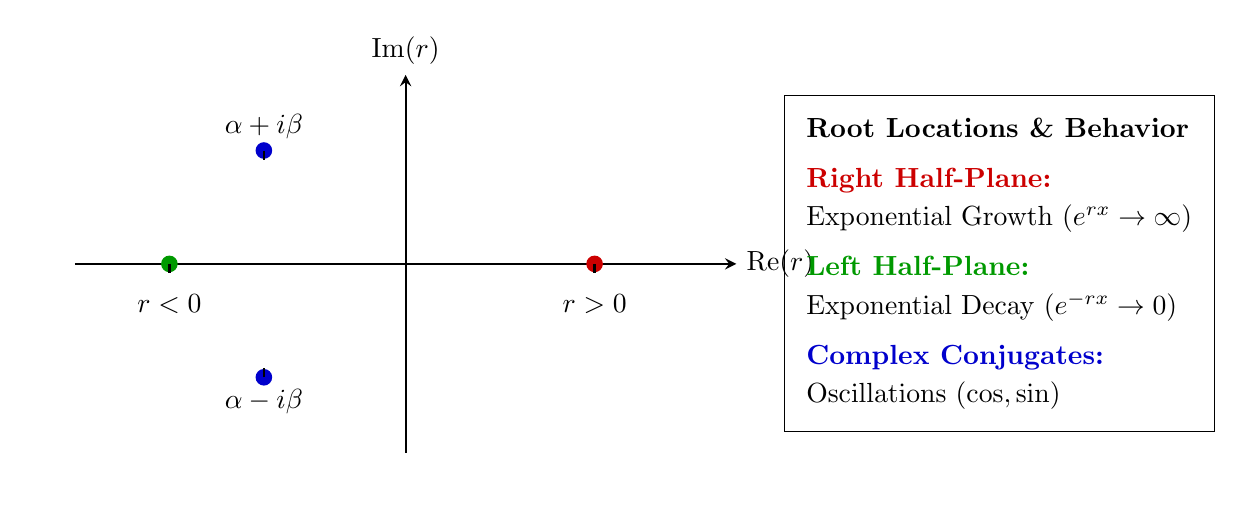
\begin{tikzpicture}[scale=1.2]
    % Background to ensure safe rendering
    \fill[white] (-4,-2.5) rectangle (4,2.5);
    
    % Axes
    \draw[thick, ->, >=stealth] (-3.5,0) -- (3.5,0) node[right] {$\text{Re}(r)$};
    \draw[thick, ->, >=stealth] (0,-2) -- (0,2) node[above] {$\text{Im}(r)$};
    
    % Roots
    \fill[blue!80!black] (-1.5, 1.2) circle (2.5pt);
    \fill[blue!80!black] (-1.5, -1.2) circle (2.5pt);
    \fill[red!80!black] (2, 0) circle (2.5pt);
    \fill[green!60!black] (-2.5, 0) circle (2.5pt);
    
    % Tick marks and labels
    \draw[thick] (-1.5, 1.2) -- (-1.5, 1.1) node[above=4pt, black] {$\alpha + i\beta$};
    \draw[thick] (-1.5, -1.2) -- (-1.5, -1.1) node[below=4pt, black] {$\alpha - i\beta$};
    \draw[thick] (2, 0) -- (2, -0.1) node[below=4pt, black] {$r > 0$};
    \draw[thick] (-2.5, 0) -- (-2.5, -0.1) node[below=4pt, black] {$r < 0$};
    
    % Legend Node
    \node[align=left, anchor=west, black, draw, inner sep=8pt] at (4, 0) {
        \textbf{Root Locations \& Behavior}\\[6pt]
        \textcolor{red!80!black}{\textbf{Right Half-Plane:}}\\[2pt]
        Exponential Growth ($e^{rx} \to \infty$)\\[6pt]
        \textcolor{green!60!black}{\textbf{Left Half-Plane:}}\\[2pt]
        Exponential Decay ($e^{-rx} \to 0$)\\[6pt]
        \textcolor{blue!80!black}{\textbf{Complex Conjugates:}}\\[2pt]
        Oscillations ($\cos, \sin$)
    };
\end{tikzpicture}
\end{center}

\subsection{B) Forward and Backward Links}
\textbf{Backward Links:} This topic is the direct, logical extension of solving first-order linear ODEs (like $y' + ky = 0$) and second-order ODEs. It generalizes the exact same characteristic equation technique to $n$-dimensions. It also relies heavily on the algebraic theory of polynomials (Fundamental Theorem of Algebra).

\textbf{Forward Links:} Mastering homogeneous equations is the absolute prerequisite for solving \textit{non-homogeneous} equations (where the right side is not zero, e.g., $L[y] = f(x)$). Techniques like the \textbf{Method of Undetermined Coefficients} and \textbf{Variation of Parameters} require you to first find the homogeneous solution ($y_c$) before finding the particular solution ($y_p$). Furthermore, this theory is the foundation for understanding \textbf{Laplace Transforms} and \textbf{Systems of Linear Differential Equations}, where the characteristic equation reappears as the eigenvalue equation $\det(A - \lambda I) = 0$.

\newpage
\section{Part 6: Abstract Real-World Modeling (AI, ML, \& Quant Finance)}

\subsection{A) Concrete Scenarios}
\begin{enumerate}
    \item \textbf{Quantitative Finance (CARMA Models):} In high-frequency algorithmic trading, asset returns and volatility are often modeled using Continuous-Time Autoregressive Moving Average (CARMA) processes. The autoregressive part of a CARMA model is governed by a higher-order linear differential equation. The roots of the characteristic polynomial determine whether the financial time series is mean-reverting (roots in the left half-plane) or explosive.
    \item \textbf{Machine Learning (Momentum Optimizers):} In training deep neural networks, optimization algorithms like Heavy Ball or Nesterov Accelerated Gradient can be modeled as second or third-order differential equations in continuous time. The "friction" or "damping" coefficients correspond to the constants in the ODE, and tuning these hyperparameters is equivalent to placing the roots of the characteristic equation to achieve critical damping (fastest convergence without oscillation).
\end{enumerate}

\subsection{B) Model Problem Setup: CARMA(3,1) Volatility Modeling}
Let us formulate a continuous-time model for the unobserved instantaneous variance $V(t)$ of an asset price process. We assume $V(t)$ follows a CARMA(3,1) process driven by a standard Brownian motion $W(t)$.

The state space is continuous time $t \ge 0$. The process is defined by the stochastic differential equation system, which can be formally written using the differential operator $D = \frac{d}{dt}$:
\[ (D^3 + a_2 D^2 + a_1 D + a_0) V(t) = (b_1 D + b_0) \dot{W}(t) \]
where $\dot{W}(t)$ is Gaussian white noise. 

To ensure that the volatility process is stationary and mean-reverting (a strict requirement in finance, as volatility cannot grow to infinity), the homogeneous part of the differential operator must be strictly stable. We analyze the unforced deterministic system:
\[ V'''(t) + a_2 V''(t) + a_1 V'(t) + a_0 V(t) = 0 \]
The characteristic equation is:
\[ P(r) = r^3 + a_2 r^2 + a_1 r + a_0 = 0 \]
For the quantitative model to be valid, we must constrain the hyperparameters $(a_2, a_1, a_0)$ such that all roots $r_1, r_2, r_3$ of $P(r)$ have strictly negative real parts ($\text{Re}(r_k) < 0$). By Routh-Hurwitz stability criteria, this requires:
\[ a_2 > 0, \quad a_0 > 0, \quad \text{and} \quad a_2 a_1 > a_0 \]
If these conditions are met, the homogeneous solution $V_h(t) = c_1 e^{r_1 t} + c_2 e^{r_2 t} + c_3 e^{r_3 t}$ decays to zero, ensuring that the stochastic process admits a stationary probability measure, allowing quants to price options using Fourier transform techniques on the resulting characteristic function.

\newpage
\section{Part 7: Common Variations and Untested Concepts}

While the homework thoroughly covered homogeneous equations with constant coefficients, standard curricula usually include two immediate extensions that were absent from this set.

\subsection{1. Non-Homogeneous Equations (Undetermined Coefficients)}
\textbf{Concept:} What if the equation is $y'' - 3y' + 2y = e^{5x}$? The right side is no longer zero. The general solution becomes $y(x) = y_c(x) + y_p(x)$, where $y_c$ is the complementary (homogeneous) solution, and $y_p$ is a particular solution guessed based on the form of the right-hand side.

\textbf{Example:} Solve $y'' - 3y' + 2y = e^{5x}$.
\begin{itemize}
    \item \textit{Step 1:} Solve homogeneous $y'' - 3y' + 2y = 0 \implies r^2 - 3r + 2 = 0 \implies (r-1)(r-2) = 0$. So, $y_c(x) = c_1 e^x + c_2 e^{2x}$.
    \item \textit{Step 2:} Guess $y_p(x) = A e^{5x}$. Then $y_p' = 5A e^{5x}$ and $y_p'' = 25A e^{5x}$.
    \item \textit{Step 3:} Substitute into the ODE: $25A e^{5x} - 3(5A e^{5x}) + 2(A e^{5x}) = e^{5x}$.
    \item \textit{Step 4:} Simplify: $(25A - 15A + 2A)e^{5x} = e^{5x} \implies 12A = 1 \implies A = \frac{1}{12}$.
    \item \textit{Final Solution:} $y(x) = c_1 e^x + c_2 e^{2x} + \frac{1}{12} e^{5x}$.
\end{itemize}

\subsection{2. Cauchy-Euler Equations (Variable Coefficients)}
\textbf{Concept:} Equations of the form $a x^2 y'' + b x y' + c y = 0$ have variable coefficients, but they are perfectly structured so that the substitution $y = x^m$ transforms them into an algebraic characteristic equation.

\textbf{Example:} Solve $x^2 y'' - 3x y' + 3y = 0$.
\begin{itemize}
    \item \textit{Step 1:} Let $y = x^m$. Then $y' = m x^{m-1}$ and $y'' = m(m-1)x^{m-2}$.
    \item \textit{Step 2:} Substitute: $x^2(m(m-1)x^{m-2}) - 3x(m x^{m-1}) + 3x^m = 0$.
    \item \textit{Step 3:} Factor out $x^m$: $x^m [m(m-1) - 3m + 3] = 0$.
    \item \textit{Step 4:} Solve the characteristic equation: $m^2 - m - 3m + 3 = 0 \implies m^2 - 4m + 3 = 0 \implies (m-1)(m-3) = 0$.
    \item \textit{Final Solution:} $y(x) = c_1 x^1 + c_2 x^3$.
\end{itemize}

\newpage
\section{Part 8: Advanced Diagnostic Testing: "Find the Flaw"}

Below are five problems with complete solutions that contain a single, critical flaw. Your task as the grader is to identify the error, explain why it is wrong in one sentence, and provide the correct solution.

\subsection*{Flawed Problem 1}
\textbf{Problem:} Find the general solution to $y'' - 6y' + 9y = 0$.
\textbf{Flawed Solution:}
The characteristic equation is $r^2 - 6r + 9 = 0$.
Factoring yields $(r - 3)^2 = 0$.
The roots are $r = 3$ and $r = 3$.
Therefore, the general solution is $y(x) = c_1 e^{3x} + c_2 e^{3x}$.

\textbf{Correction Task:}
\begin{itemize}
    \item \textbf{Error:} The solution fails to multiply the second term by $x$ for a repeated root, making the two terms linearly dependent.
    \item \textbf{Correct Solution:} $y(x) = c_1 e^{3x} + c_2 x e^{3x}$.
\end{itemize}

\subsection*{Flawed Problem 2}
\textbf{Problem:} Find the general solution to $y'' + 25y = 0$.
\textbf{Flawed Solution:}
The characteristic equation is $r^2 + 25 = 0$.
Solving for $r$, we get $r^2 = 25$, so $r = \pm 5$.
The general solution is $y(x) = c_1 e^{5x} + c_2 e^{-5x}$.

\textbf{Correction Task:}
\begin{itemize}
    \item \textbf{Error:} The square root of $-25$ is $\pm 5i$, not $\pm 5$, which means the solution should involve trigonometric functions, not real exponentials.
    \item \textbf{Correct Solution:} $r = \pm 5i \implies y(x) = c_1 \cos(5x) + c_2 \sin(5x)$.
\end{itemize}

\subsection*{Flawed Problem 3}
\textbf{Problem:} Find the general solution to $y''' - y'' = 0$.
\textbf{Flawed Solution:}
The characteristic equation is $r^3 - r^2 = 0$.
Factoring out $r^2$, we get $r^2(r - 1) = 0$.
The roots are $r = 0$ (multiplicity 2) and $r = 1$.
The general solution is $y(x) = c_1 e^{0x} + c_2 e^{0x} + c_3 e^x = c_1 + c_2 + c_3 e^x$.

\textbf{Correction Task:}
\begin{itemize}
    \item \textbf{Error:} The repeated root $r=0$ requires the second term to be multiplied by $x$, otherwise $c_1$ and $c_2$ just collapse into a single constant.
    \item \textbf{Correct Solution:} $y(x) = c_1 + c_2 x + c_3 e^x$.
\end{itemize}

\subsection*{Flawed Problem 4}
\textbf{Problem:} Find the general solution to $y'' - 4y' + 13y = 0$.
\textbf{Flawed Solution:}
The characteristic equation is $r^2 - 4r + 13 = 0$.
Using the quadratic formula: $r = \frac{4 \pm \sqrt{16 - 52}}{2} = \frac{4 \pm \sqrt{-36}}{2} = \frac{4 \pm 6i}{2} = 2 \pm 3i$.
The general solution is $y(x) = c_1 \cos(3x) + c_2 \sin(3x)$.

\textbf{Correction Task:}
\begin{itemize}
    \item \textbf{Error:} The real part of the complex root ($\alpha = 2$) was omitted; it must appear as an exponential multiplier $e^{2x}$.
    \item \textbf{Correct Solution:} $y(x) = e^{2x}(c_1 \cos(3x) + c_2 \sin(3x))$.
\end{itemize}

\subsection*{Flawed Problem 5}
\textbf{Problem:} Solve the IVP: $y'' - y = 0$, with $y(0)=1, y'(0)=1$.
\textbf{Flawed Solution:}
Characteristic equation: $r^2 - 1 = 0 \implies r = \pm 1$.
General solution: $y(x) = c_1 e^x + c_2 e^{-x}$.
Derivative: $y'(x) = c_1 e^x + c_2 e^{-x}$.
At $x=0$: $c_1 + c_2 = 1$ and $c_1 + c_2 = 1$.
This system has infinitely many solutions, so we can just pick $c_1 = 1, c_2 = 0$.
Final answer: $y(x) = e^x$.

\textbf{Correction Task:}
\begin{itemize}
    \item \textbf{Error:} The derivative of $e^{-x}$ is $-e^{-x}$ (chain rule), which changes the second equation to $c_1 - c_2 = 1$, yielding a unique solution.
    \item \textbf{Correct Solution:} $y'(x) = c_1 e^x - c_2 e^{-x}$. The system is $c_1 + c_2 = 1$ and $c_1 - c_2 = 1$. Adding them gives $2c_1 = 2 \implies c_1 = 1$, and $c_2 = 0$. The final answer $y(x) = e^x$ happens to be correct by sheer luck, but the calculus step and logical justification were fundamentally flawed.
\end{itemize}

\end{document}